\documentclass[tikz,border=3pt]{standalone}
\usepackage[utf8]{inputenc}
\usepackage[T1]{fontenc}
\usepackage{lmodern}
\renewcommand{\familydefault}{\sfdefault}
\usepackage{sansmath}\sansmath
\usepackage{chemfig}
\usepackage{pgfplots}\pgfplotsset{compat=1.18,/pgf/number format/use comma,/pgf/number format/1000 sep={.}}
\usetikzlibrary{arrows.meta,calc,positioning,decorations.pathmorphing,patterns}
% paleta del sitio
\definecolor{nar}{HTML}{E8680C}\definecolor{narc}{HTML}{FFB35C}\definecolor{hielo}{HTML}{FFF3E8}
\definecolor{tinta}{HTML}{1D1D1F}\definecolor{gris}{HTML}{6E6E73}\definecolor{lila}{HTML}{7C5CF0}
\definecolor{azul}{HTML}{2F6FD6}\definecolor{menta}{HTML}{17A673}\definecolor{coral}{HTML}{E8342A}
\tikzset{cel/.style={draw=gris,fill=hielo,line width=0.9pt},nuc/.style={draw=gris!70,line width=0.6pt},
fib/.style={gris!55,line width=0.35pt},eti/.style={font=\footnotesize,text=tinta,align=center},
num/.style={circle,draw=nar,fill=white,text=nar,font=\small\bfseries,inner sep=1.2pt,minimum size=13pt},
fl/.style={-{Stealth[length=2.6mm]},gris,line width=0.9pt}}
\begin{document}
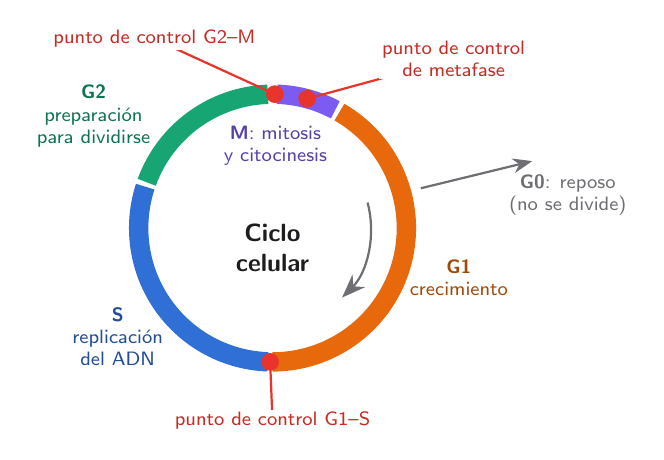
\begin{tikzpicture}[font=\small]
\draw[nar,line width=7pt] (0.85,1.472) arc (60:-90:1.7);
\draw[azul,line width=7pt] (-0.059,-1.699) arc (-92:-198:1.7);
\draw[menta,line width=7pt] (-1.597,0.581) arc (-200:-268:1.7);
\draw[lila,line width=7pt] (0.059,1.699) arc (88:62:1.7);
\draw[-{Stealth[length=3mm]},gris,line width=0.8pt] (1.207,0.324) arc (15:-45:1.25);
\node[font=\small\bfseries,text=tinta,align=center] at (0,-0.25) {Ciclo\\celular};
\node[font=\scriptsize,text=nar!70!black,align=center] at (2.367,-0.634) {\textbf{G1}\\crecimiento};
\node[font=\scriptsize,text=azul!70!black,align=center] at (-1.966,-1.377) {\textbf{S}\\replicación\\del ADN};
\node[font=\scriptsize,text=menta!70!black,align=center] at (-2.273,1.42) {\textbf{G2}\\preparación\\para dividirse};
\node[font=\scriptsize,text=lila!70!black,align=center] at (0.037,1.049) {\textbf{M}: mitosis\\y citocinesis};
\draw[-{Stealth[length=2.5mm]},gris,thick] (1.884,0.505)--(3.3,0.85);
\node[font=\scriptsize,text=gris,align=center] at (3.75,0.42) {\textbf{G0}: reposo\\(no se divide)};
\draw[coral,thick] (-0.03,-1.7)--(0,-2.45);
\fill[coral] (-0.03,-1.7) circle (3.2pt);
\node[font=\scriptsize,text=coral!85!black,fill=white,inner sep=1pt,align=center] at (0,-2.45) {punto de control G1–S};
\draw[coral,thick] (0.03,1.7)--(-1.5,2.4);
\fill[coral] (0.03,1.7) circle (3.2pt);
\node[font=\scriptsize,text=coral!85!black,fill=white,inner sep=1pt,align=center] at (-1.5,2.4) {punto de control G2–M};
\draw[coral,thick] (0.44,1.642)--(2.3,2.15);
\fill[coral] (0.44,1.642) circle (3.2pt);
\node[font=\scriptsize,text=coral!85!black,fill=white,inner sep=1pt,align=center] at (2.3,2.15) {punto de control\\de metafase};
\end{tikzpicture}
\end{document}
